%#! platex  -halt-on-error -file-line-error -src-specials main.tex
% Time-stamp: <2016-12-14 19:48:32 takago>


% F3: タイプセット.
% F4: エラー箇所へ.
% F5: プレビュー. xdvi上で [CTRL]を押しながら左クリックを押すと,その付近にジャンプする.

\documentclass[25pt, landscape,dvipdfmx]{foils}
\usepackage{color}
\usepackage{graphicx}
\usepackage{fancyhdr}
%
\special{papersize=297mm,210mm}  % papersize=width, height
%
\topmargin = -25mm
\oddsidemargin = -10mm
\evensidemargin = -10mm
\textheight = 175mm
\textwidth = 270mm
%
\headheight=10mm
\footskip=15mm
%
\LogoOff
%
%\pagestyle{plain}
%%%%%%%%%%%% setup of the footer %%%%%%%%%%%%%
\pagestyle{fancy}
\renewcommand{\headrulewidth}{0pt}
\renewcommand{\footrulewidth}{0pt}
\lfoot{}
\cfoot{}
\rfoot{{\footnotesize 最小自乗法を用いた画素ごとの局所適応予測符号化法 \hskip10mm \thepage/\pageref{LastPage}}} 


%
%
%%%%%%%%%%%% thickness of the line around fboxes %%%%%%%%
\setlength{\fboxrule}{1.5pt}
%
%
%%%%%%%%%%%%%%%%%%%%%%%%%%%%%%%%%%%%%%%%%
%%%
%%%  日本語フォントをゴシックに、数式フォントを太字に変更する
%%%
\renewcommand{\kanjifamilydefault}{\gtdefault}
\mathversion{bold}

\title{\vspace{2cm}最小自乗法を用いた\\画素ごとの局所適応予測符号化法} 
\date{2007年9月13日}
\author{
武田 晴信\\
武田 信繁\\
武田 信廉\\
}


\MyLogo{} 
%\rightfooter{quad\textsf{\thepage}}   % this is the default
\setlength{\foilheadskip}{0mm}
\setlength{\parindent}{0mm}
%%%%%%%%%%%%%%%%%%%

\begin{document}
\maketitle
%%%%%%%%%%%%
\foilhead[-14mm]{\Large 発表の流れ}
\begin{enumerate}
 \item 画像の予測符号化とは
 \item 最小自乗法を用いた従来の予測符号化手法
 \item 画素適応予測符号化法
 \item むすび
\end{enumerate}
      
%%%%%%%%%%%%
\foilhead[-14mm]{\Large 1. 画像の予測符号化とは}
\begin{itemize}
 \item ああああ
 \item 無損失圧縮法の一つ
       \begin{itemize}
        \item 各画素値をその周辺の画素値から予測し,その誤差(予測誤差)を符号化する.
        \item 復号化は符号化と同じ予測を行って得られた予測値に予測誤差を加える.
       \end{itemize}
 \item 予測に用いる予測式係数の決定法
 \begin{itemize}
  \item 固定式
  \item 最小自乗法
 \end{itemize}
\end{itemize}
%%%%%%%%%%%%
\foilhead[-14mm]{\Large 2. 最小自乗法を用いた従来の予測符号化手法}
\begin{itemize}
 \item {\large ブロック適応法・・・ブロックごとに予測式係数を算出}\\
       注目ブロック内の符号化(復号化)が済んでいない画素も利用
 \begin{itemize}
  \item 予測係数の次数が大きいとオーバーヘッド大
 \end{itemize}
 \item {\large 画素適応法・・・画素ごとに予測式係数を算出}\\
       符号化(復号化)済みの画素だけを利用
 \begin{itemize}
  \item 予測係数のオーバーヘッド不要
  \item 計算量が膨大
 \end{itemize}
\end{itemize}
%%%%%%%%%%%%%%%%%%%%%%%
\foilhead[-14mm]{\Large 3. 画素適応予測符号化法}
\begin{figure}
\begin{center}
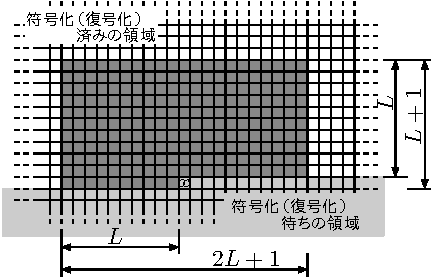
\includegraphics[width=20.5cm]{fig/fig2.pdf}
%\vspace{5mm}\\
\end{center}
{\small 注目画素$x$の上部のグレー領域が予測式係数決定に使われる領域(参照領域)\\
参照領域の大きさを示すパラメータ:$L$}
\end{figure}
\newpage
\begin{figure}[b]
\begin{center}
\vspace{-1cm}
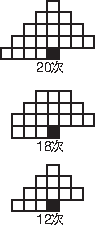
\includegraphics[scale=2]{fig/yosokusiki.pdf}
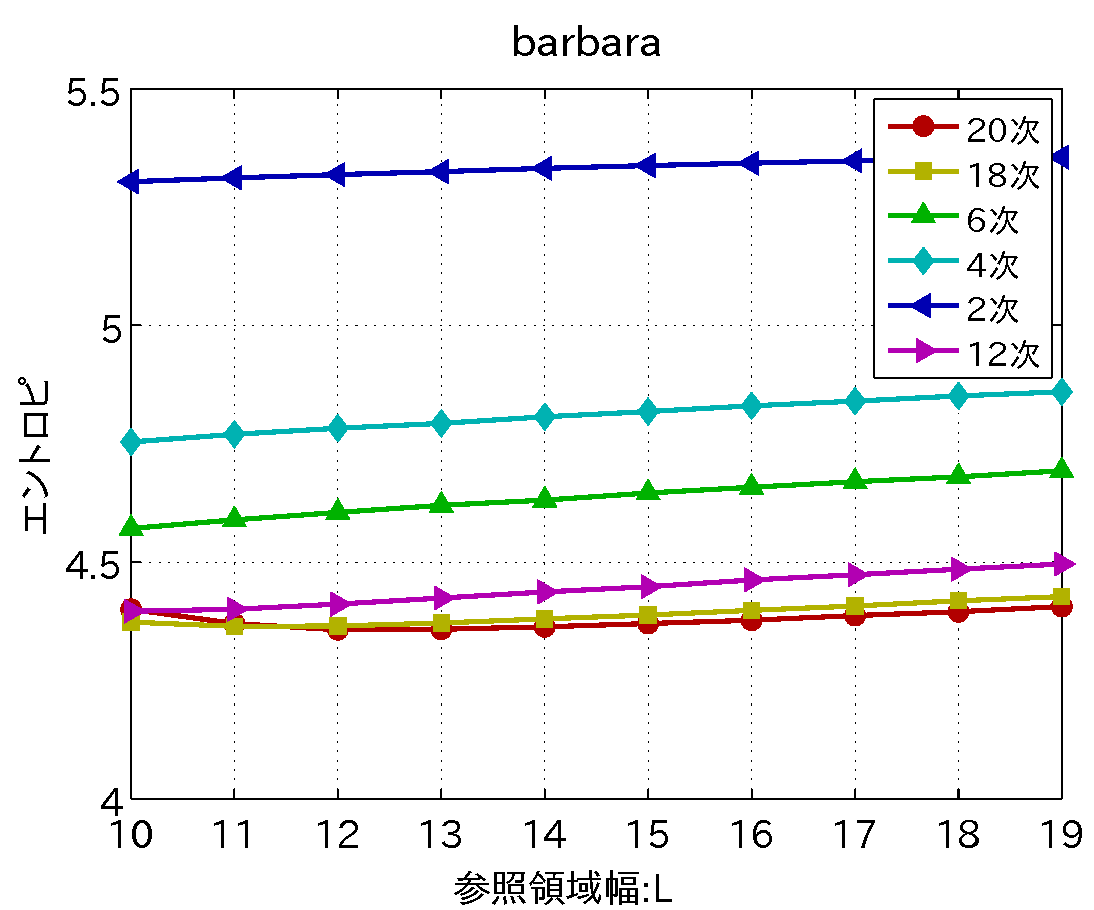
\includegraphics[width=11.5cm]{fig/test1/barbara.pdf}
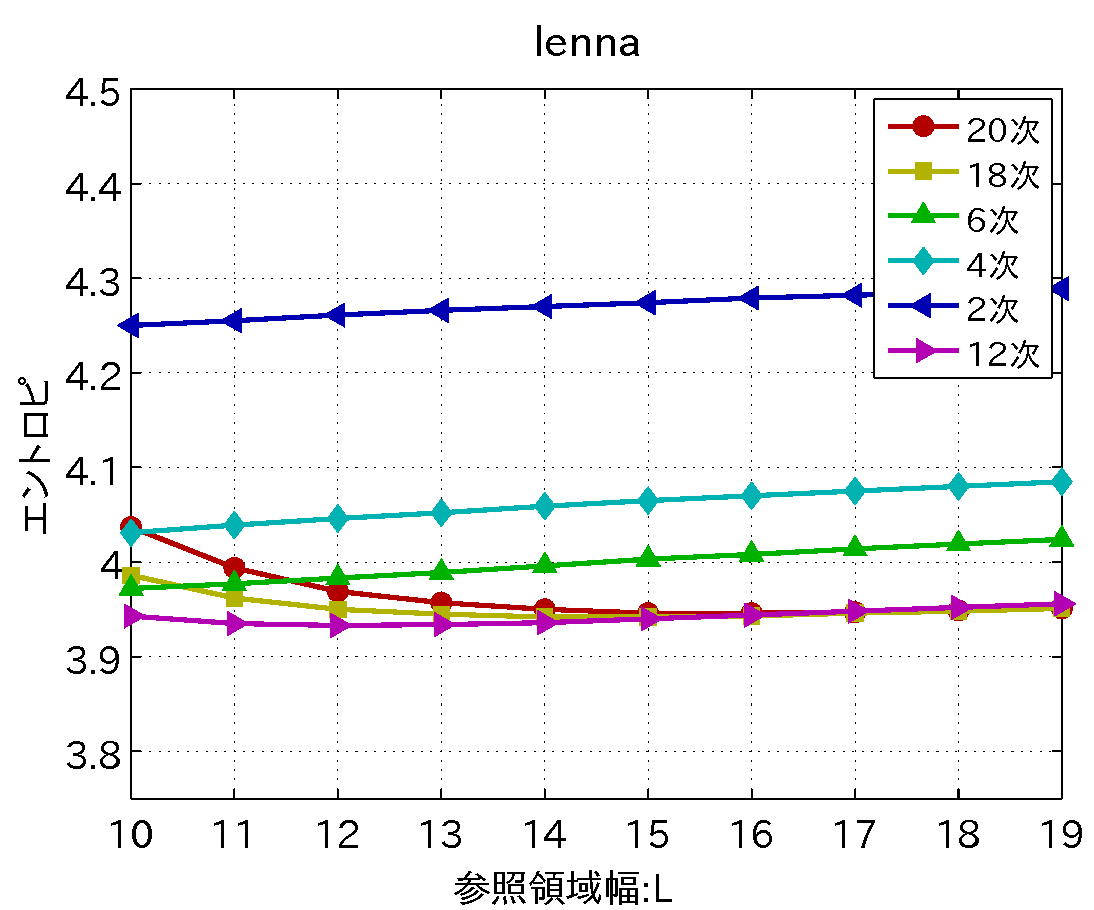
\includegraphics[width=11.5cm]{fig/test1/lenna.pdf}\\
\vspace{3mm}
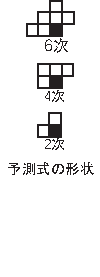
\includegraphics[scale=2]{fig/yosokusiki2.pdf}
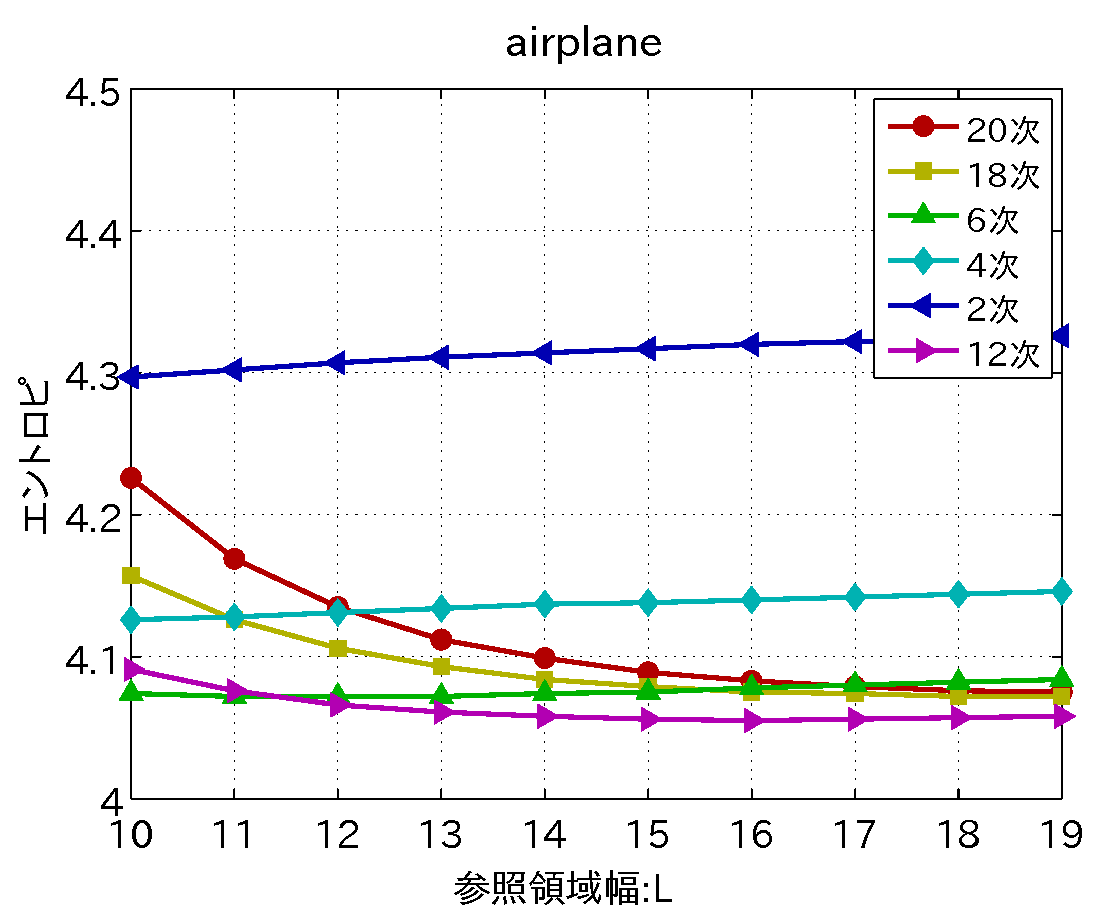
\includegraphics[width=11.5cm]{fig/test1/airplane.pdf}
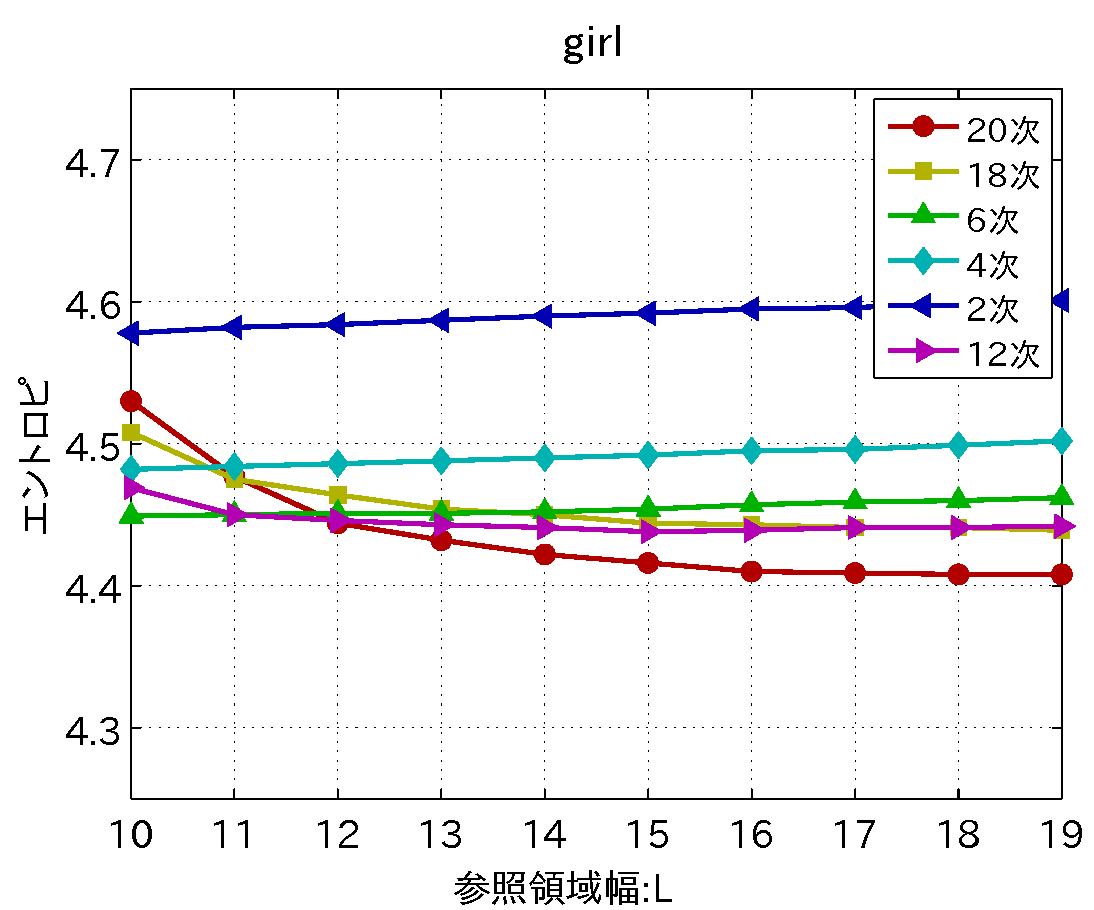
\includegraphics[width=11.5cm]{fig/test1/girl.pdf}
%\caption{予測式の形状$p$, 左から$p=0,1,2,3,4,5$とする}
\end{center}
\end{figure}
%%%%%%%%%%%%
\newpage
局所的に予測式の形状や参照領域の大きさ$L$を変えると,予測誤差がより小さくなるのでは?
\begin{center}
$\Downarrow$
\end{center}
\fbox{\Large ブロックごとの画素適応予測}
\begin{itemize}
\item \large 画素ごとに予測式係数を算出し,ブロックごとに予測誤差の自乗和が最小となる様な,
\begin{itemize}
  \item 予測式の形状($2,4,6,12,18,20$次)
  \item 参照領域サイズ($L=10,11,12,\cdots,19$)
 \end{itemize}
を選択(わずかなオーバーヘッド)\\
\end{itemize}

%%%%%%%%%%%%
\newpage

\begin{figure}[b]
\begin{flushleft}
\vspace{-1cm}
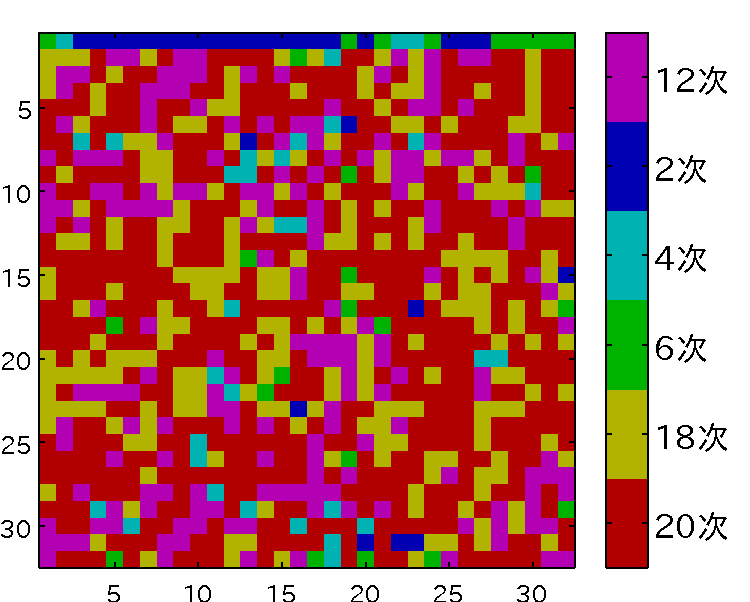
\includegraphics[angle=-90,scale=0.75]{fig/test1/b16/yosokusikino.pdf}
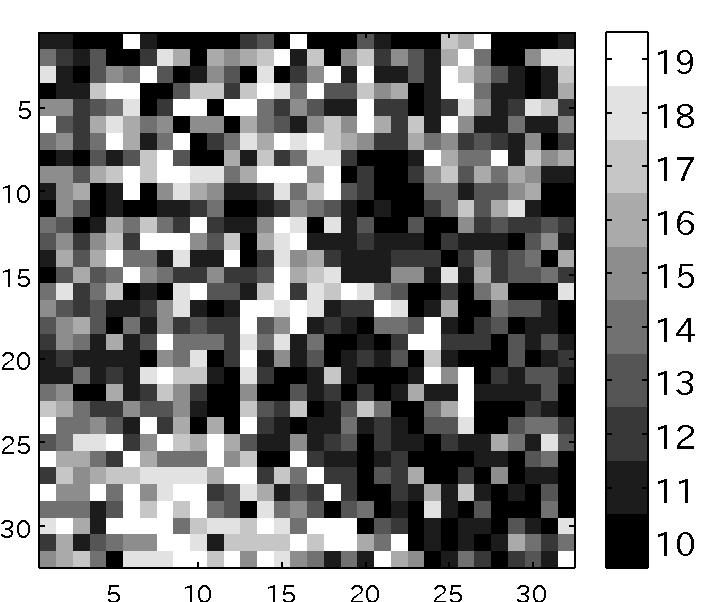
\includegraphics[angle=-90,scale=0.75]{fig/test1/b16/yosokusikihaba.pdf}
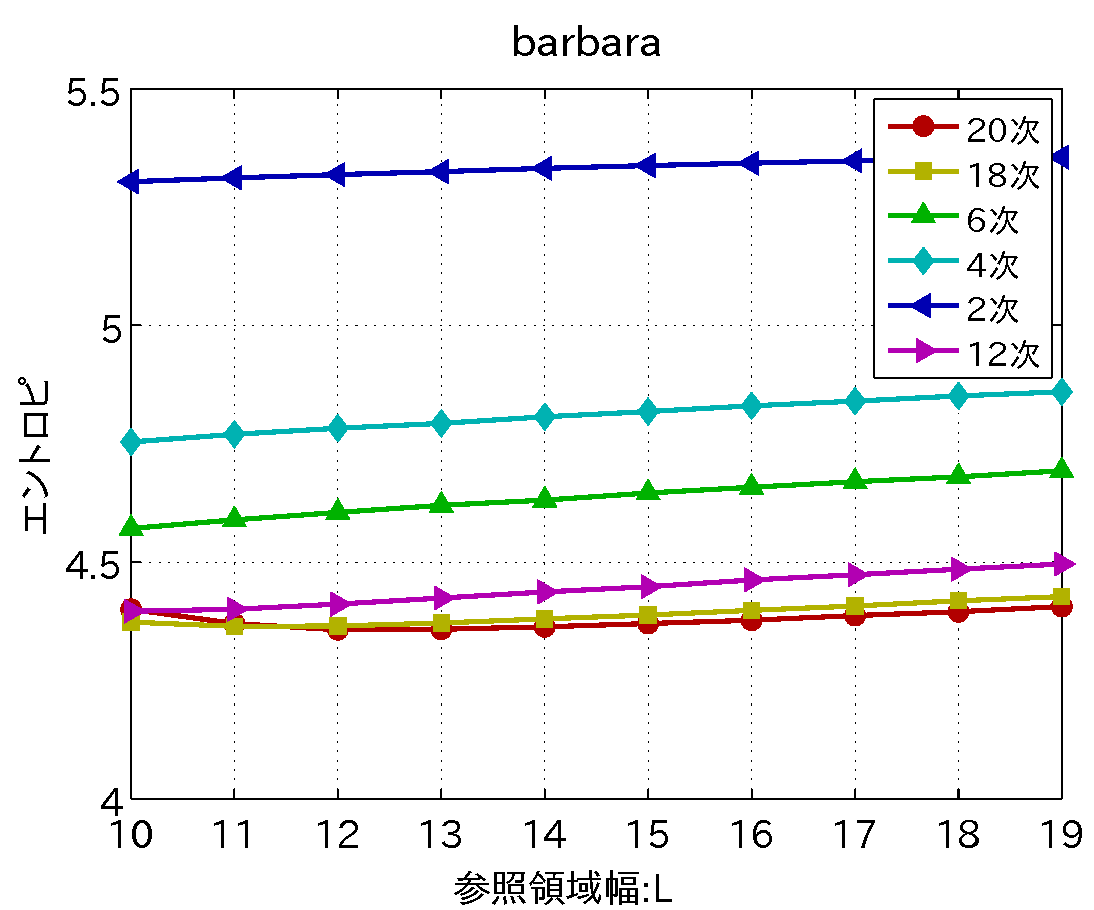
\includegraphics[scale=0.75]{fig/test1/barbara.pdf}\\
\vspace{3mm}
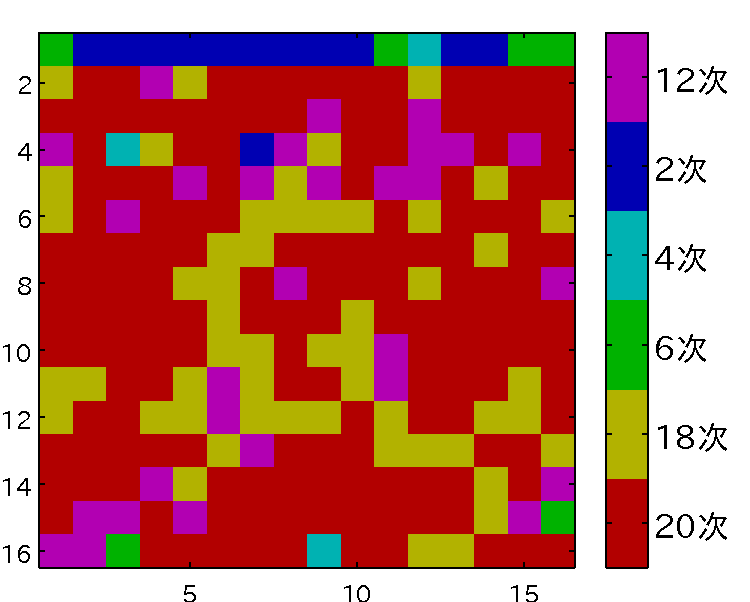
\includegraphics[angle=-90,scale=0.75]{fig/test1/b32/yosokusikino.pdf}
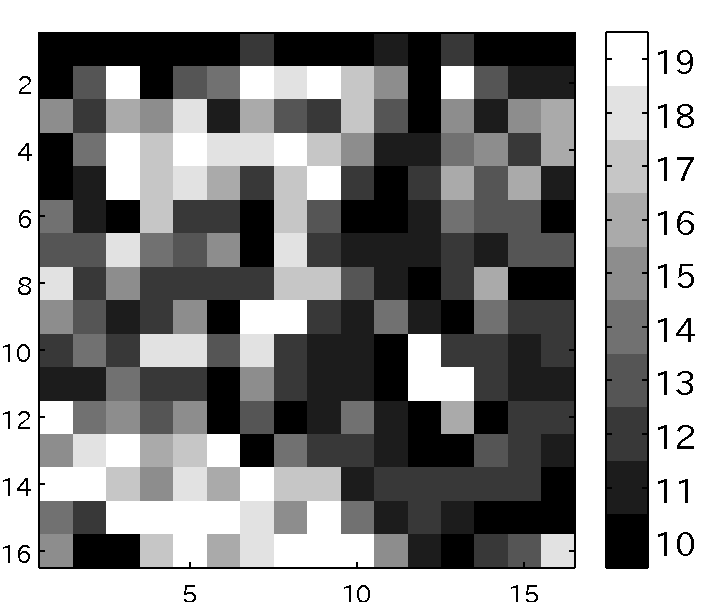
\includegraphics[angle=-90,scale=0.75]{fig/test1/b32/yosokusikihaba.pdf}\\
予測誤差の自乗和を最小化する予測式の形状と参照領域幅
上段$16^2$pel/BK,下段$32^2$pel/BK,画像はbarbara(右上端)
\end{flushleft}
\end{figure}
%%%%%%%%%%%%
\newpage
\begin{figure}[b]
\begin{flushleft}
\vspace{-1cm}
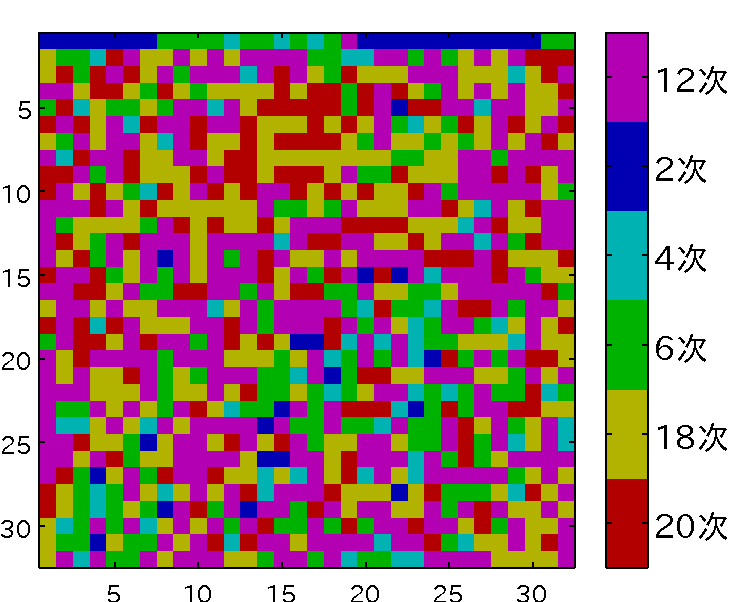
\includegraphics[angle=-90,scale=0.75]{fig/test1/l16/yosokusikino.pdf}
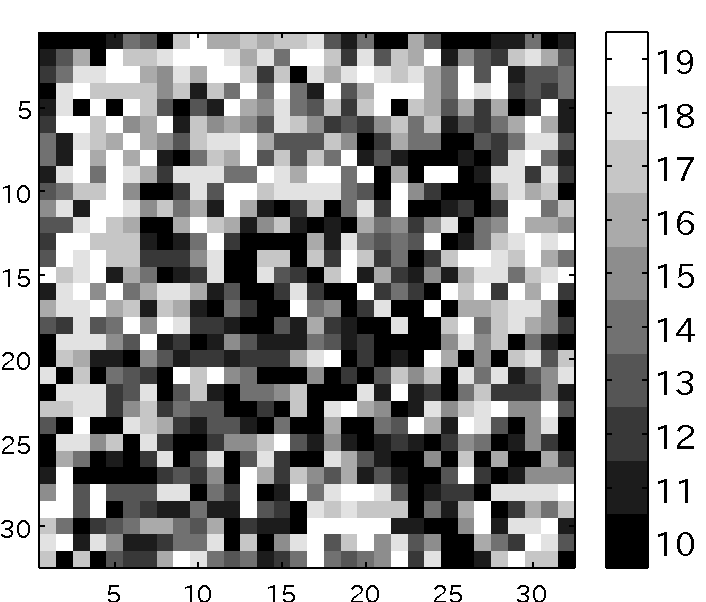
\includegraphics[angle=-90,scale=0.75]{fig/test1/l16/yosokusikihaba.pdf}
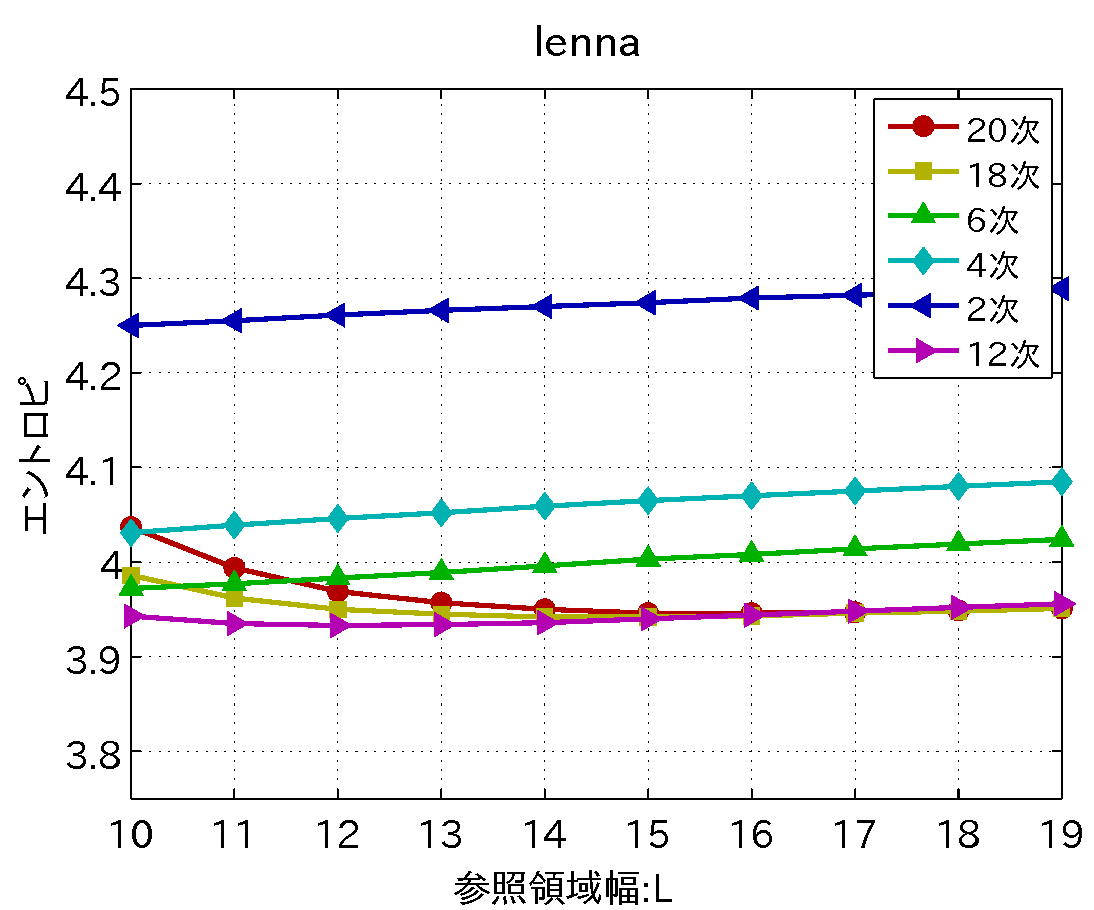
\includegraphics[scale=0.75]{fig/test1/lenna.pdf}\\
\vspace{3mm}
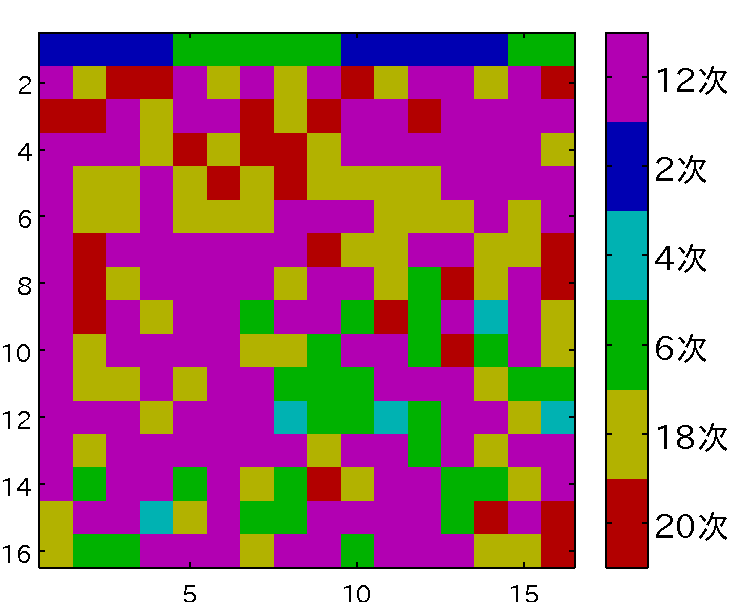
\includegraphics[angle=-90,scale=0.75]{fig/test1/l32/yosokusikino.pdf}
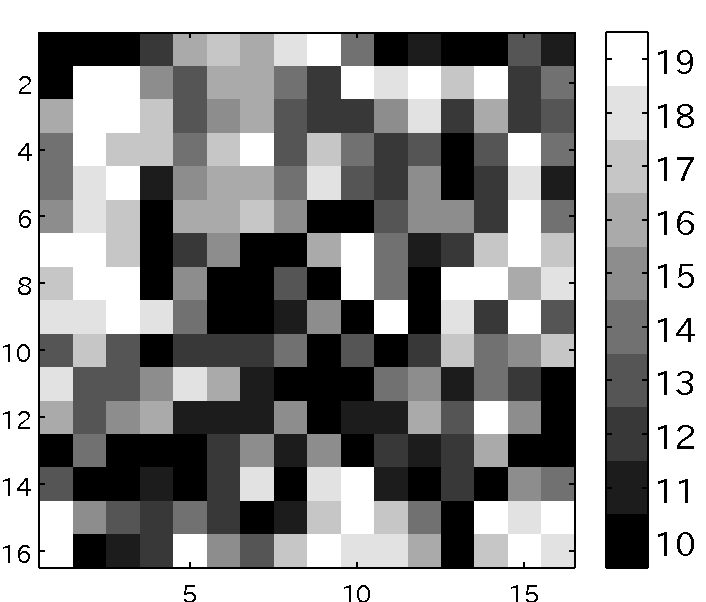
\includegraphics[angle=-90,scale=0.75]{fig/test1/l32/yosokusikihaba.pdf}\\
予測誤差の自乗和を最小化する予測式の形状と参照領域幅\\
上段$16^2$pel/BK,下段$32^2$pel/BK,画像はlenna(右上端)
\end{flushleft}
\end{figure}
\newpage
\begin{table}[h]
\begin{center}
{\large 5種の画像に対する予測誤差のエントロピ($^*$は平均符号長)}
\vspace{8mm}
\begin{tabular}{l|cccc|cc}
\noalign{\hrule height 1pt}
画像& $16^2$pel/BK & $32^2$pel/BK&20次&12次&LOCO-I$^*$&CALIC$^*$\\
\noalign{\hrule height 1pt} 
barbara &4.314&4.331&4.406&4.496& 4.885 &	4.702 \\
        &(4.291)&(4.325)&&&\\\hline
lenna   &3.913&3.915&3.951&3.956& 4.016 &	3.903 \\
        &(3.890)&(3.909)&&&\\\hline
airplane&4.021&4.027&4.075&4.058& 3.820 &	3.742 \\
        &(3.998)&(4.021)&&&\\\hline
peppers &4.426&4.442&4.491&4.491& 4.511 &	4.424 \\
        &(4.403)&(4.436)&&&\\\hline
girl    &4.368&4.373&4.408&4.442& 4.542 &	4.431 \\
        &(4.345)&(4.367)&&&\\
\noalign{\hrule height 1pt}
\end{tabular}\\
\end{center}
\small 尚,括弧内の数値はオーバーヘッドを含めないときのエントロピを示す.\\''20次'',''12次''は画素適応予測の結果で$L=19$の場合を示す.
\end{table}

%%%%%%%%%%%%
\foilhead[-14mm]{\Large 4. むすび}

 \begin{itemize}
  \item {\large } 5種の標準画像でブロックごとの画素適応予測の有効性が確認出来た.
  \begin{itemize}
   \item $16\times16$画素を1ブロックとした方法では,20次の画素適応予測の結果より0.038--0.091エントロピが小さい.
  \end{itemize}
  \item 今後の課題
  \begin{itemize}
   \item 予測誤差を元にしたコンテクストクラスのレンジコーディング
   \item 重みつき最小自乗法の導入
   \begin{itemize}
    \item 注目画素から離れた部分の影響を抑制(画素適応予測に限り可能)
   \end{itemize}
  \end{itemize}
 \end{itemize}
\end{document} 
